\documentclass[UTF8,11pt,fontset=fandol]{ctexart}
\usepackage[a4paper,top=21mm,bottom=22mm,left=23mm,right=23mm]{geometry}
\usepackage{amsmath,amssymb,amsthm,mathtools}
\usepackage{tikz,booktabs,array,enumitem,fancyhdr}
\usepackage[hidelinks,pdfauthor={数学解答},pdftitle={2026高联预赛A卷加试解答}]{hyperref}
\usetikzlibrary{calc,angles,quotes}
\setlength{\headheight}{14pt}
\pagestyle{fancy}
\fancyhf{}
\fancyhead[L]{\small 2026 高联预赛 A 卷}
\fancyhead[R]{\small 加试解答}
\fancyfoot[C]{\thepage}
\setlength{\parskip}{4pt}
\linespread{1.18}
\setlist[enumerate]{leftmargin=2em,itemsep=3pt,topsep=3pt}
\numberwithin{equation}{section}
\ctexset{section={format=\Large\bfseries,number=\chinese{section}、,aftername={}}}
\newcommand{\problem}{\noindent\textbf{题目\quad}}
\newcommand{\solution}{\par\medskip\noindent\textbf{解答\quad}}
\newcommand{\step}[1]{\par\medskip\noindent\textbf{#1}\par}
\newcommand{\qedmark}{\qed\par}

\begin{document}
\begin{center}
  {\LARGE\bfseries 2026 高联预赛 A 卷加试解答}\par
  \vspace{5pt}
  {\small 对应本项目试卷 PDF 第二页的四道加试题}
\end{center}

\section{正约数中的等差数列}
\problem
设 $1=d_1<d_2<\cdots<d_m=n$ 是正整数 $n$ 的所有正约数，$m\ge4$。
对任意 $i,j\in\{1,\ldots,m-1\}$，均存在 $k\in\{1,\ldots,m\}$，
使 $d_i,d_j,d_k$ 在某种顺序下构成等差数列。求 $m$ 的所有可能值。

\solution 答案为 $\boxed{m=4}$。

设 $p$ 是 $n$ 的最小素因子，$L=n/p$ 是 $n$ 的最大真约数。
由于 $m\ge4$，$n$ 是合数，故 $L\ge p$；并且 $L\ge3$。

对真约数 $1,L$ 应用题设。能够与它们组成等差数列的第三个数只能是
\[
 2-L,\qquad \frac{L+1}{2},\qquad 2L-1.
\]
其中 $2-L<0$，不可能是正约数。如果 $2L-1\mid n=pL$，由
\[
 \gcd(2L-1,L)=1
\]
可得 $2L-1\mid p$，但 $2L-1>L\ge p$，矛盾。因此只能有
\[
 L\text{ 为奇数},\qquad \frac{L+1}{2}\mid pL.
\]
又因为
\[
 \gcd\!\left(\frac{L+1}{2},L\right)=1,
\]
故 $(L+1)/2\mid p$。它大于 $1$，而 $p$ 为素数，所以
\[
 \frac{L+1}{2}=p,\qquad L=2p-1,\qquad n=p(2p-1).
\]

下面证明 $2p-1$ 是素数。否则，它的每个素因子都是 $n$ 的素因子，
因而不小于 $p$，从而 $2p-1\ge p^2$；这与 $p^2>2p-1$ 矛盾。
由于 $2p-1>p$，$n$ 是两个不同素数的乘积，因此 $m=4$。

最后验证 $m=4$ 确实可以出现：取 $n=6$，其真约数为 $1,2,3$。
任意两个不同的真约数都可与剩下的一个组成等差数列；当 $i=j$ 时，
取 $k=i$ 即得到公差为 $0$ 的等差数列。故题设全部满足。\qedmark

\newpage
\section{斜边中点、九点圆与相切}
\problem
在锐角三角形 $ABC$ 中，$AB<AC$，$AD$ 是 $BC$ 边上的高，
$H$ 为垂心，$O$ 为外心，$N$ 为 $HO$ 的中点。
线段 $BD$ 内一点 $P$ 满足 $\angle PND=2\angle PAD$。
证明：直线 $BC$ 与三角形 $AOP$ 的外接圆相切。

\solution
\textbf{取 $AP$ 的中点 $E$，连接 $DE,EN$。}
记 $\alpha=\angle PAD$。在直角三角形 $ADP$ 中，斜边中点给出 $EA=ED=EP$，故
\[
 \angle DEP=2\angle EAD=2\angle PAD=\angle DNP.
\]
由于 $E,N$ 同在直线 $DP$ 的 $A$ 侧，故 $D,E,N,P$ 四点共圆，记此圆为 $\omega$。
这里 $AB<AC$ 保证 $BC$ 的中点位于 $D$ 的 $C$ 侧，因而 $O,N$ 与 $E$
分居直线 $AD$ 两侧，特别地 $N\ne E$。

由 $ED=EP$，$E$ 位于弦 $DP$ 的垂直平分线上，所以
\textbf{$\omega$ 在 $E$ 处的切线 $\ell$ 平行于 $BC$}。

\begin{center}
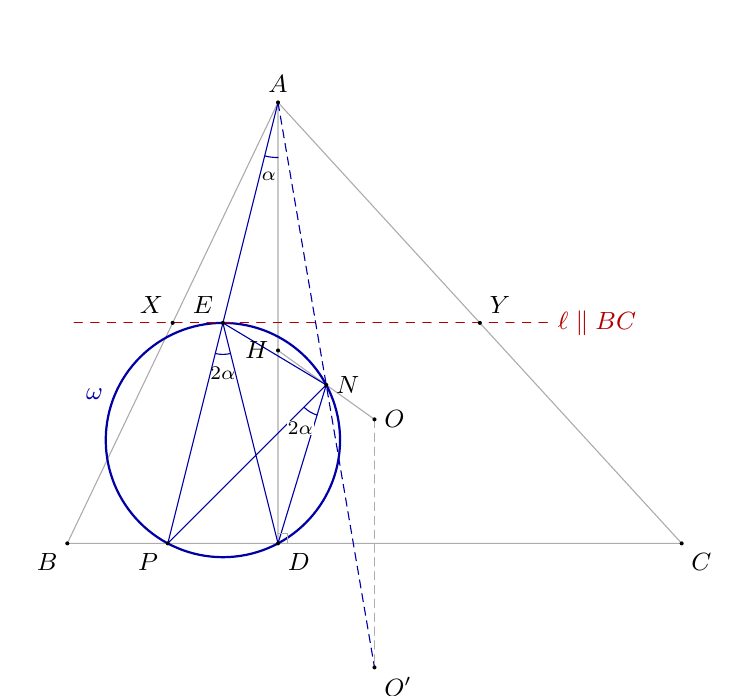
\begin{tikzpicture}[scale=.70,line cap=round,line join=round,
  every node/.style={font=\small}]
  % The chosen configuration satisfies the given angle condition exactly.
  \coordinate (A) at (0,8);
  \coordinate (B) at ({(7-sqrt(497))/4},0);
  \coordinate (C) at ({(7+sqrt(497))/4},0);
  \coordinate (D) at (0,0);
  \coordinate (P) at (-2,0);
  \coordinate (E) at (-1,4);
  \coordinate (X) at ($(A)!.5!(B)$);
  \coordinate (Y) at ($(A)!.5!(C)$);
  \coordinate (H) at (0,{7/2});
  \coordinate (O) at ({7/4},{9/4});
  \coordinate (Op) at ({7/4},{-9/4});
  \coordinate (N) at ({7/8},{23/8});
  \draw[gray!65] (A)--(B)--(C)--cycle (A)--(D) (H)--(O);
  \draw[blue!65!black,densely dashed] (A)--(Op);
  \draw[gray!65,densely dashed] (O)--(Op);
  \draw[blue!65!black,thick] (-1,{15/8}) circle[radius={17/8}];
  \draw[blue!65!black] (A)--(P) (P)--(N)--(D) (D)--(E)--(N);
  \draw[red!70!black,dashed] (-3.7,4)--(4.9,4) node[right] {$\ell\parallel BC$};
  \pic[draw=blue!65!black,angle radius=7mm,angle eccentricity=1.35,
    "$\alpha$"{font=\scriptsize}] {angle=P--A--D};
  \pic[draw=blue!65!black,angle radius=4mm,angle eccentricity=1.6,
    "$2\alpha$"{font=\scriptsize}] {angle=P--E--D};
  \pic[draw=blue!65!black,angle radius=4mm,angle eccentricity=1.6,
    "$2\alpha$"{font=\scriptsize,fill=white,inner sep=.3pt}] {angle=P--N--D};
  \draw[gray!65] (0,.18)--(.18,.18)--(.18,0);
  \foreach \Q in {A,B,C,D,P,E,X,Y,H,O,Op,N}{\fill (\Q) circle[radius=1.05pt];}
  \node[above] at (A) {$A$};
  \node[below left] at (B) {$B$};
  \node[below right] at (C) {$C$};
  \node[below right] at (D) {$D$};
  \node[below left] at (P) {$P$};
  \node[above left] at (E) {$E$};
  \node[above left] at (X) {$X$};
  \node[above right] at (Y) {$Y$};
  \node[left] at (H) {$H$};
  \node[right] at (O) {$O$};
  \node[below right] at (Op) {$O'$};
  \node[right] at (N) {$N$};
  \node[blue!65!black,left] at (-3,2.7) {$\omega$};
\end{tikzpicture}
\par\small $X,E,Y$ 分别为 $AB,AP,AC$ 的中点，同在红色虚线 $\ell$ 上；
\par\small $O'$ 为 $O$ 关于 $BC$ 的对称点，蓝色圆 $\omega$ 与 $\ell$ 相切于 $E$。
\end{center}

现在考虑变换 $\mathcal T$：\textbf{先关于 $BC$ 反射，再以 $A$ 为中心作比为 $1/2$ 的位似}。
设 $X,Y$ 分别为 $AB,AC$ 的中点。显然
\[
 \mathcal T(A)=D,\qquad \mathcal T(B)=X,\qquad
 \mathcal T(C)=Y,\qquad \mathcal T(P)=E.
\]
因此，$\mathcal T$ 把 $\triangle ABC$ 的外接圆变为经过 $D,X,Y$ 的九点圆。
九点圆的圆心正是 $HO$ 的中点 $N$，而反射、位似都把圆心映为圆心，故
\[
 \mathcal T(O)=N.
\]
这也说明图中的 $N$ 是 $AO'$ 的中点。

于是，$\mathcal T$ 把 $\triangle AOP$ 的外接圆变为 $\omega$，
把直线 $BC$ 变为过 $E$ 且平行于 $BC$ 的直线，即 $\ell$。
已知 $\omega$ 与 $\ell$ 相切于 $E$，将变换逆向还原，便知
\textbf{$\triangle AOP$ 的外接圆与 $BC$ 相切于 $P$}。\qedmark

\newpage
\section{首尾配对与余量补偿}
\problem
设整数 $n>100$，实数 $2\ge a_0\ge a_1\ge\cdots\ge a_{n-1}\ge0$。
对任意 $0\le i\le j\le k\le n-1$ 且 $i+j+k\ge n$，均有
\[
 a_i a_j+a_j a_k+a_k a_i\le a_i+a_j+a_k.
\]
证明：
\[
 \text{(1)}\quad \sum_{i=1}^{n-1}a_i\le n-1;
 \qquad
 \text{(2)}\quad \sum_{i=0}^{n-1}a_i\le n.
\]

\solution
\textbf{首尾配对，再用中间四对的余量补足首项。}
先注意：若 $3r\ge n$，在题设中取三个指标均为 $r$，得到
$3a_r^2\le3a_r$，因而 $0\le a_r\le1$。

\step{(1) 每一对的和不超过 $2$}
任取 $1\le i\le j\le n-1$ 且 $i+j=n$。由于 $2i+j\ge n$，
将 $(i,i,j)$ 代入题设，并利用 $j\ge n/2$ 时 $a_j\le1$，得
\[
 (a_i+a_j)^2
 \le 2a_i+a_j+a_j^2
 \le2(a_i+a_j).
\]
因此 $a_i+a_j\le2$。把 $a_1,\ldots,a_{n-1}$ 首尾配对；若有剩余的中间一项，
其指标为 $n/2$，也不超过 $1$。于是
\[
 \boxed{\sum_{i=1}^{n-1}a_i\le n-1}.
\]

\step{(2) 中间四对各节省首项超额的四分之一}
若 $a_0\le1$，结论由 (1) 立即得到。以下设 $u=a_0-1\in(0,1]$。

对任意 $j\ge n/2$，令 $t=1-a_j\ge0$。
将 $(0,j,j)$ 代入题设，有 $a_j^2+2a_0a_j\le a_0+2a_j$。
代入 $a_j=1-t$ 并整理，利用 $a_0\le2$，得到
\[
 u\le2a_0t-t^2\le4t,
 \qquad\text{所以}\qquad
 a_j\le1-\frac u4.
\]

再看 (1) 中的配对，\textbf{取最靠近中间的四对}。
由于 $n>100$，这四对都存在，而且每一对的较小指标 $i$、较大指标 $j$ 满足
\[
 i\ge\frac n2-4>\frac n3,\qquad j\ge\frac n2.
\]
因此 $a_i\le1$，$a_j\le1-u/4$，即这四对中的每一对都有
\[
 a_i+a_j\le 2-\frac u4.
\]
其余各对的和仍不超过 $2$，若有中间单独一项则不超过 $1$。
四对共节省 $u$，故 (1) 可加强为
\[
 \sum_{i=1}^{n-1}a_i\le n-1-u.
\]
加上 $a_0=1+u$，即得
\[
 \boxed{\sum_{i=0}^{n-1}a_i\le n}.
\]
当所有 $a_i=1$ 时，题设成立且两问同时取等号。\qedmark

\newpage
\section{\texorpdfstring{$4\times n$ 方格表中的 $S$ 形}{4×n 方格表中的 S 形}}
\problem
在 $4\times n$（$n\ge2$）方格表中填入非负实数。
每个 $S$ 形的四格之和均不小于 $1$，其中允许的四种形状如下（可平移）：
\begin{center}
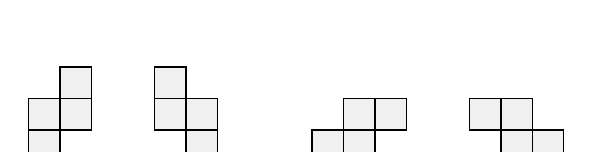
\begin{tikzpicture}[x=4mm,y=4mm,line width=.5pt]
\foreach \dx/\type in {0/1,4/2,9/3,14/4}{
  \begin{scope}[shift={(\dx,0)}]
  \ifnum\type=1
    \foreach \x/\y in {0/0,0/1,1/1,1/2}{\draw[fill=gray!12] (\x,\y) rectangle +(1,1);}
  \fi
  \ifnum\type=2
    \foreach \x/\y in {1/0,1/1,0/1,0/2}{\draw[fill=gray!12] (\x,\y) rectangle +(1,1);}
  \fi
  \ifnum\type=3
    \foreach \x/\y in {0/0,1/0,1/1,2/1}{\draw[fill=gray!12] (\x,\y) rectangle +(1,1);}
  \fi
  \ifnum\type=4
    \foreach \x/\y in {0/1,1/1,1/0,2/0}{\draw[fill=gray!12] (\x,\y) rectangle +(1,1);}
  \fi
  \end{scope}
}
\end{tikzpicture}
\end{center}
求全表所有数之和的最小值。

\solution
最小值为：$n$ 为奇数时 $\boxed{n-1}$；$n$ 为偶数时 $\boxed{\dfrac{n^2}{n+1}}$。
记全表总和为 $T$，行、列分别从上到下、从左到右编号。

\medskip\noindent\textbf{(i) $n=2k+1$。}
在上两行取 $k$ 个横向 $S$ 形：第 $r$ 个占第 $1$ 行的第 $2r,2r+1$ 格，
以及第 $2$ 行的第 $2r-1,2r$ 格；下两行同样取 $k$ 个。
这 $2k$ 个 $S$ 形互不重叠，故 $T\ge2k=n-1$。
偶数列全填 $1/2$、奇数列全填 $0$ 时，每个 $S$ 形恰有两格为 $1/2$，等号成立。

\medskip\noindent\textbf{(ii) $n=2k$。}
记中间两行的总和为 $I$。将列分为 $k$ 对 $(1,2),(3,4),\ldots,(n-1,n)$。
每对列中的四个竖向 $S$ 形全部相加，外侧两行各格计一次，中间两行各格计三次，故
\begin{equation}\label{eq:vertical-count}
 T+2I\ge4k=2n.
\end{equation}
对第 $r$ 对列，记其中间四格的和为 $I_r$。删去这四格及全表四个角格，
其余部分可铺成 $n-2$ 个互不重叠的横向 $S$ 形：上两行在缺口两侧反向错开一格，
分别铺 $r-1$ 个、$k-r$ 个；下两行作上下对称的铺放。例如 $n=8,r=2$ 时，上两行为
\[
\begin{array}{cccccccc}
 \cdot&A&A&B&B&C&C&\cdot\\
 A&A&\cdot&\cdot&B&B&C&C
\end{array}
\quad\text{（同字母四格为一个 $S$ 形，点号为删去的格子）}.
\]
由非负性，$T-I_r\ge n-2$。对 $r=1,\ldots,k$ 求和，利用 $\sum I_r=I$，得
\begin{equation}\label{eq:horizontal-count}
 kT-I\ge k(n-2).
\end{equation}
将 \eqref{eq:vertical-count} 加上 \eqref{eq:horizontal-count} 的两倍，消去 $I$，即得
\[
 (n+1)T\ge2n+2k(n-2)=n^2.
\]

为取到等号，先在第 $2r-1,2r$ 两列填入整数块
\[
 \begin{pmatrix}
 r-1&k-r\\
 r&k-r+1\\
 r&k-r+1\\
 r-1&k-r
 \end{pmatrix}
 \qquad(r=1,\ldots,k).
\]
竖向 $S$ 形的左端列为奇、偶数时，四格之和分别为 $2k+1,2k+3$；
横向 $S$ 形位于第 $1,2$ 行或第 $3,4$ 行时为 $2k+1$，位于第 $2,3$ 行时为 $2k+3$。
每块总和为 $4k$，故将全表各数除以 $2k+1$，即得总和为
$4k^2/(2k+1)=n^2/(n+1)$ 的可行填法。
（$n=2$ 时横向铺法为空，上述论证仍成立。）\qedmark

\end{document}
